\chapter{Plan for Future Work}\label{chap:futureplan}

\section{Code for Evaluation of Multiview Models}
In support of the work in this report I have a general framework in a published software package described in chapter \ref{sec:ccazoo}. In addition I have gathered together many of the toy datasets in multiview learning literature including datasets in computer vision (MNIST, cars from different angles), natural language (matched words and an associate image from 6 languages), as well as a Twitter dataset and the canonical X-Ray Microbeam dataset. In estimating the times to complete the projects below I have accounted for this work even though it isn't in this report.

\section{Data}
In support of all of the projects, one objective is to get access to and prepare a number of real datasets. For this reason we consider the work required separately to the projects.

\subsection{UK Biobank (UKBB)}

\begin{itemize}
    \item Complete application and process files (1 month)
\end{itemize}

\subsection{Genetic Frontotemporal dementia Initiative (GENFI)}

\begin{itemize}
    \item Apply for access and process files (1 month)
\end{itemize}

\section{A General Framework for Regularised and Deep CCA based on Alternating Optimisation}
\subsection{\textbf{Contribution 1:} Alternating regularised regressions for flexible multiview learning}

\begin{itemize}
    \item Run experiments on ADNI,HCP, UKBB data demonstrating the use of Total Variation regularisation for MRI data as well as l1-norm regularisation (1 month)
    \item Work out generalisation bounds potentially with a co-author (2 months)
\end{itemize}

\section{Efficient and Non-Linear Solutions to CCA and PLS by Gradient Descent}

\subsection{\textbf{Contribution 1:} PLS Game}
\begin{itemize}
    \item Could be applied to the ADNI, HCP, UKBB data described earlier. In particular, noone in the literature has modelled Brain and Genetics data using PLS on the UK Biobank scale. We would hope to improve on the approximation in \cite{altmannpartial} in terms of the quality of the associations found (0.5 months)
\end{itemize}

\subsection{\textbf{Contribution 2:} CCA Game}
\begin{itemize}
    \item Continue to work on the mathematical problem
    \item Possible external collaborator for further analysis
\end{itemize}

\subsection{\textbf{Contribution 3:} A novel form for Deep CCA}
\begin{itemize}
    \item Run experiments on typical toy datasets (0.5 months)
    \item Run experiments on UK Biobank/ADNI (large medical datasets) to discover new non-linear associations between neuroimaging and other modalities such as behaviour and genetics (0.5 months)
\end{itemize}

\section{Identifying Multiview Effects in Subsets of a Population}

This project is at the most exploratory end of the spectrum and therefore there is a degree of uncertainty. The immediate task is:

\begin{itemize}
    \item Explore the types of data containing subgroups for which classical PCA, PLS, and CCA fail and use this knowledge to iteratively develop methods which solve these problems.
\end{itemize}

If the contributions developed so far can be modified or applied to particular data where they are effective then applications include:

\subsection{\textbf{Contribution 1 and 2:} Maximum Margin Robots for Dimensionality Reduction in the Presence of Outliers and An Improved Sparse Weighted CCA}
\begin{itemize}
    \item Run experiments on UK Biobank/ADNI/GENFI where the goal is to identify strong effects in subgroups. Where there is a ground truth like the GENFI data we can validate the model (0.5 months)
\end{itemize}

\section{Project Gant Chart}

\begin{figure}[ht]
\centerline{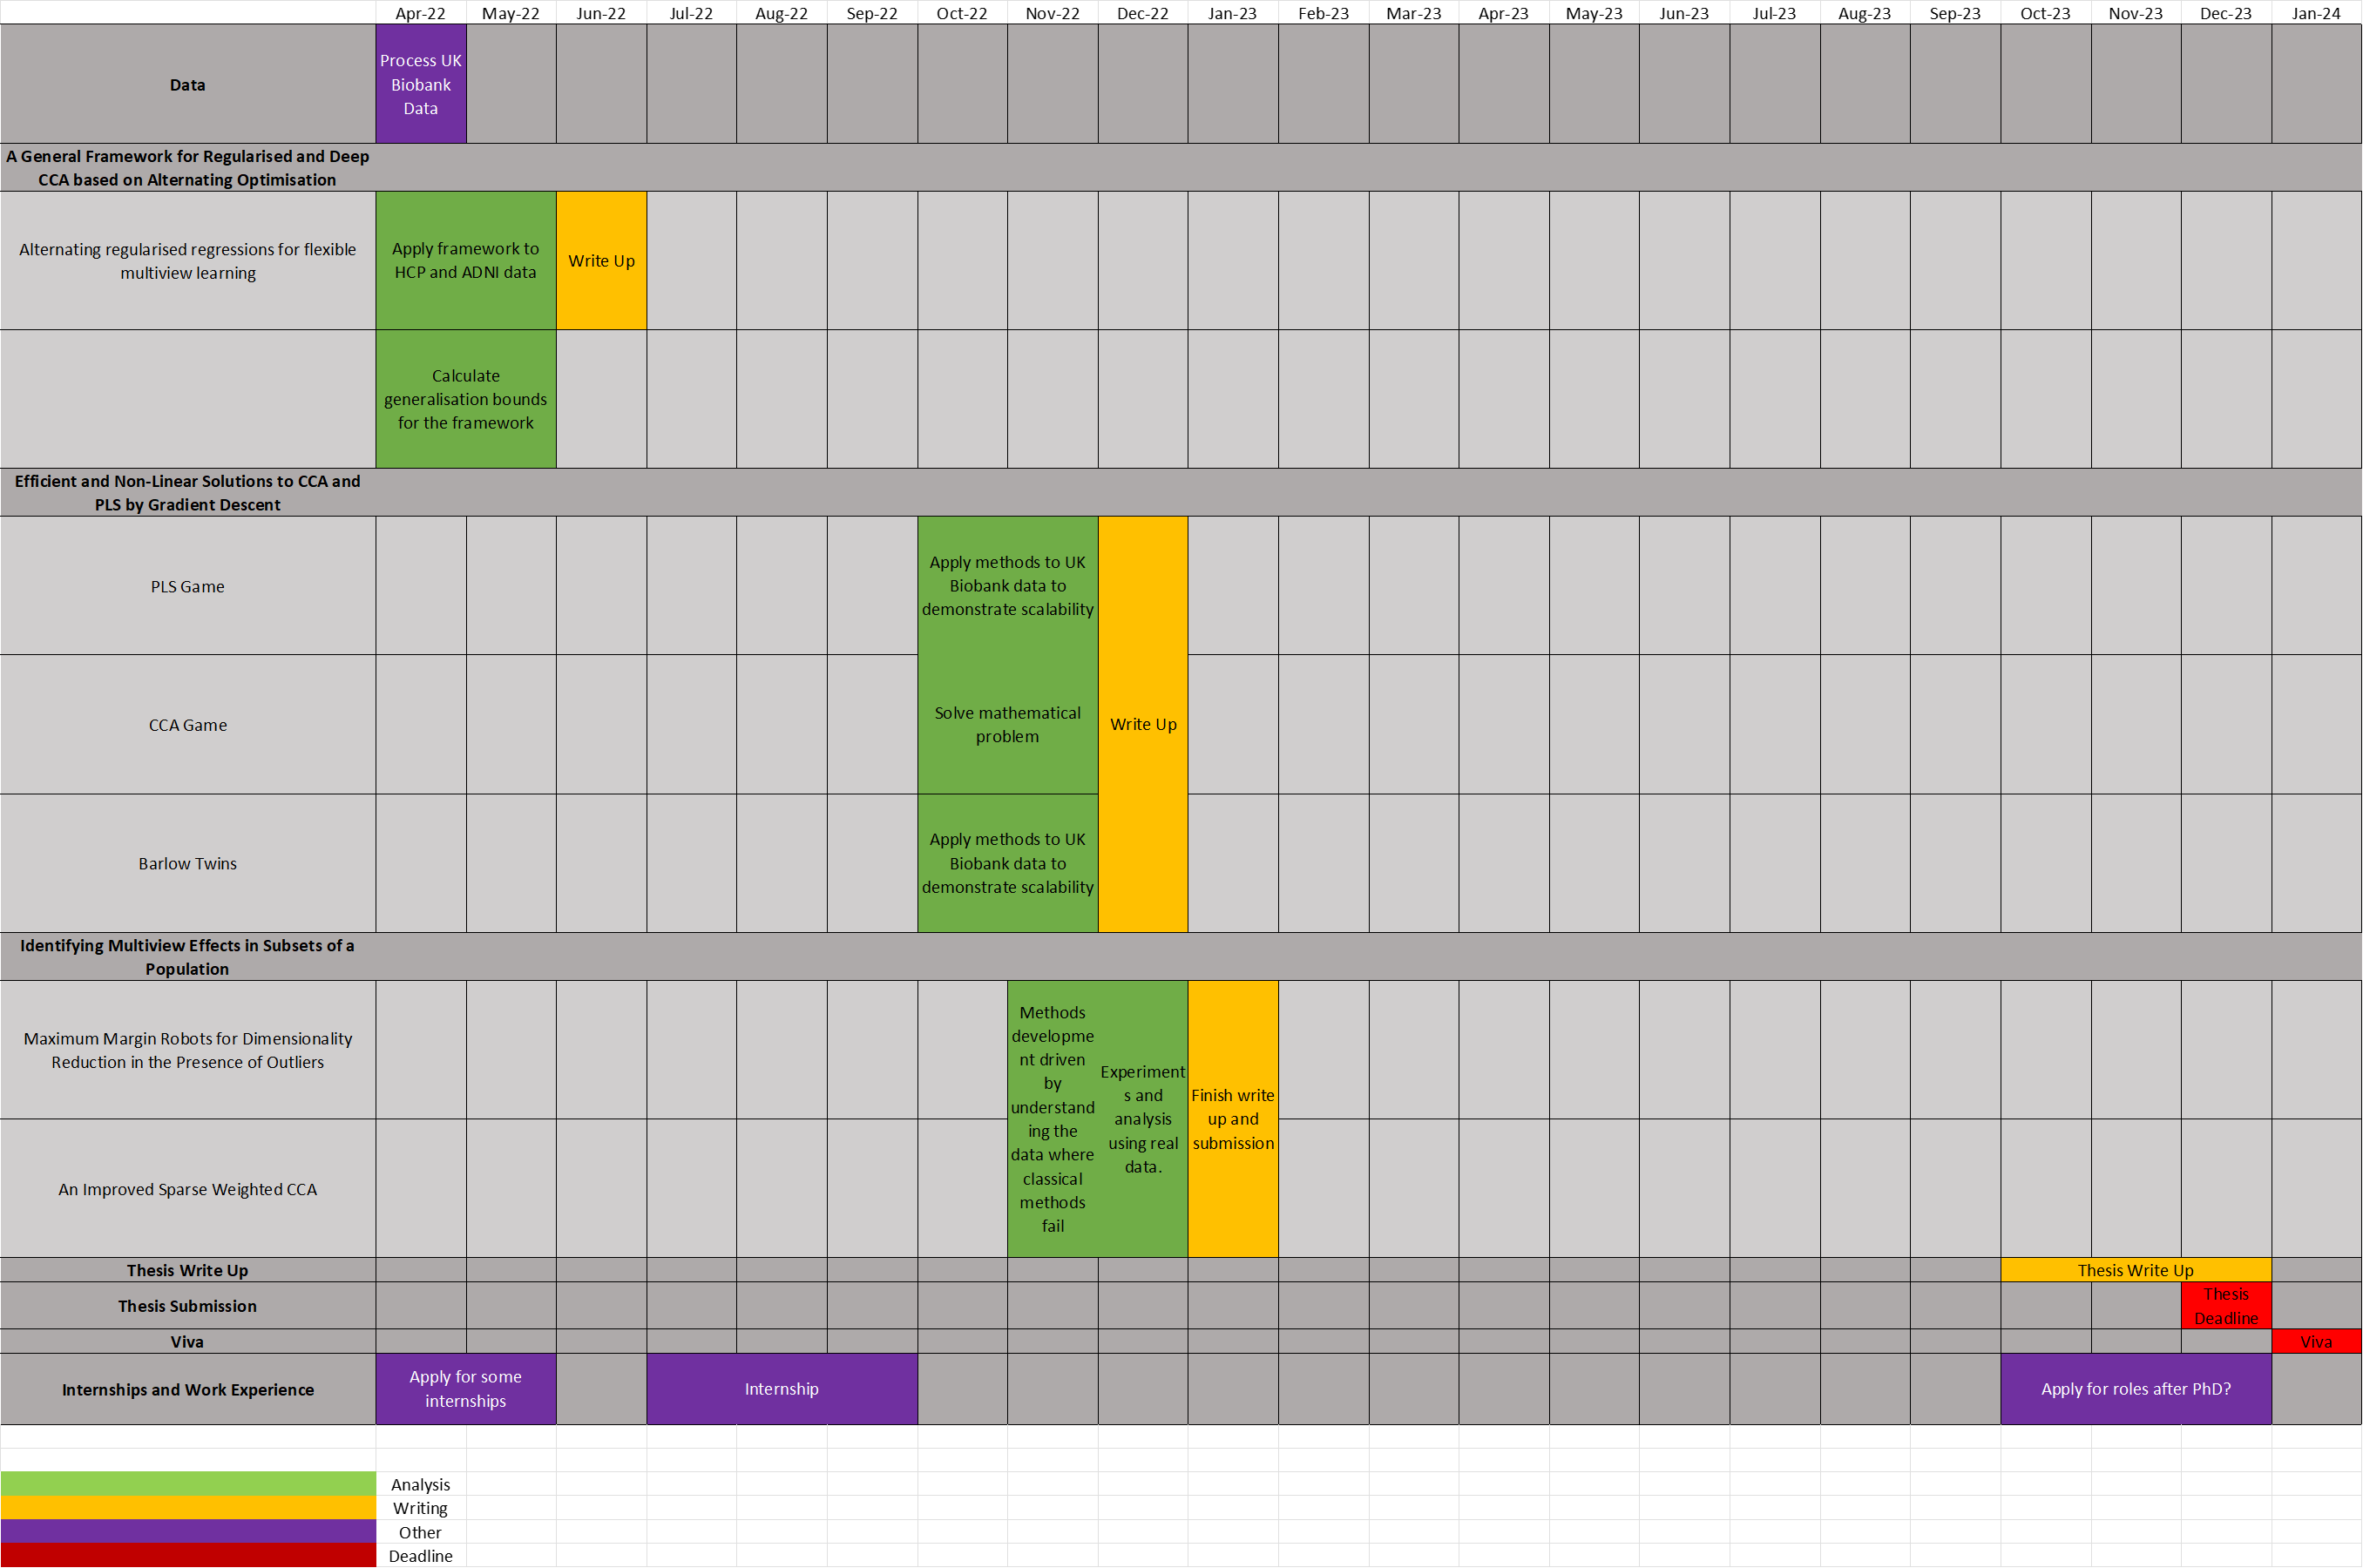
\includegraphics[width=\columnwidth]{chapters/futurework/PhDGant.png}}
\caption{A Gant Chart to illustrate intended future work from the upgrade report to the remainder of project funding}
\label{icml-historical}
\end{figure}